\documentclass{standalone}
\usepackage{graphicx}	
\usepackage{amssymb, amsmath}
\usepackage{color}

\usepackage{tikz}
\usetikzlibrary{intersections, backgrounds, math}
\usepackage{pgfmath}

\definecolor{light}{RGB}{220, 188, 188}
\definecolor{mid}{RGB}{185, 124, 124}
\definecolor{dark}{RGB}{143, 39, 39}
\definecolor{highlight}{RGB}{180, 31, 180}
\definecolor{gray10}{gray}{0.1}
\definecolor{gray20}{gray}{0.2}
\definecolor{gray30}{gray}{0.3}
\definecolor{gray40}{gray}{0.4}
\definecolor{gray60}{gray}{0.6}
\definecolor{gray70}{gray}{0.7}
\definecolor{gray80}{gray}{0.8}
\definecolor{gray90}{gray}{0.9}
\definecolor{gray95}{gray}{0.95}

\begin{document}

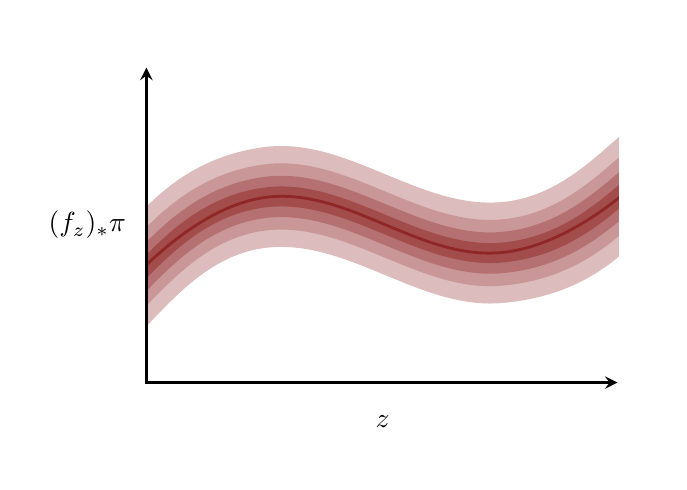
\begin{tikzpicture}[scale=1]
  \draw[white] (-4.5, -3) rectangle (3.5, 2.5);

  \begin{scope}
    \clip (-3, -2) rectangle (3, 2);
    \foreach [count=\n] \i in {1.2815516, 0.8416212, 0.5244005, 0.2533471} {
      \pgfmathsetmacro{\prop}{25 * (\n - 1)};
      \colorlet{custom}{dark!\prop!light};
      \pgfmathsetmacro{\dy}{0.5 * \i}
      \fill[custom] 
         plot [smooth cycle, tension=0.75] coordinates { 
           (-3.5, -1 + \dy) (-1.5, 0.35 + \dy) (1.5, -0.35 + \dy) (3.5, 0.75 + \dy) 
           (3.5, 0.75 - \dy) (1.5, -0.35 - \dy) (-1.5, 0.35 - \dy) (-3.5, -1 - \dy) };
    }
    
    \draw[dark, line width=1] plot [smooth, tension=0.75] coordinates { (-3.5, -1.05) (-1.5, 0.35) (1.5, -0.35) (3.5, 0.8) };
  \end{scope}

  \node at (-3.75, 0) { $(f_{z})_{*} \pi$ };

  \draw [->, >=stealth, line width=1] (-3.015, -2) -- +(6, 0);
  \draw [->, >=stealth, line width=1] (-3, -2) -- +(0, 4);
  \node at (0, -2.5) { $z$ };
  
\end{tikzpicture}

\end{document}  